\chapter{Thuật toán DFS (tìm kiếm theo chiều sâu)}
\ifpdf
    \graphicspath{{Chapter3/Chapter3Figs/PNG/}{Chapter3/Chapter3Figs/PDF/}{Chapter3/Chapter3Figs/}}
\else
    \graphicspath{{Chapter3/Chapter3Figs/EPS/}{Chapter3/Chapter3Figs/}}
\fi


\section{Giới thiệu thuật toán}
DFS hay còn được gọi là tìm kiếm ưu tiên theo chiều sâu, tìm kiếm theo chiều sâu là một thuật toán duyệt trên một cây hoặc đồ thị. Thuật toán sẽ khởi đầu tại gốc hoặc một đỉnh bất kì (đỉnh này được xem như là gốc) và phát triển xa nhất có thể theo mỗi nhánh của gốc đó.\\
DFS là một dạng tìm kiếm thjoong tin không đầy đủ bởi vì quá trình tìm kiếm được phát triển tới đỉnh con đầu tiên của nút đang tìm kiếm cho tới khi gặp được đỉnh cần tìm hoặc tới một nút không có con. Khi đó giải thuật quay lui về đỉnh vừa mới tìm kiếm ở bước trước. Trong dạng không đệ quy, tất cả các đỉnh chờ được phát triển được bổ sung vào một ngăn xếp LIFO.
\\ Xét về độ phức tạp, theo không gian DFS sẽ thấp hơn BFS nhưng sẽ tương đương nhau khi xét về thời gian.
\section{Mô tả thuật toán}
Như hình dưới đây, thuật toán DFS sẽ bắt đầu tại đỉnh A và đi theo cạnh trái và tiếp tục tìm kiếm cho đến khi hết phần nhánh cây trái rồi mới chuyển sang nhanh con bên phải. Thứ tự sau khi chạy đủ thuật toán sẽ như sau: A, B, D, F,  C, G, E.\\

\begin{figure}[!htbp]
  \begin{center}
    \leavevmode
    \ifpdf
      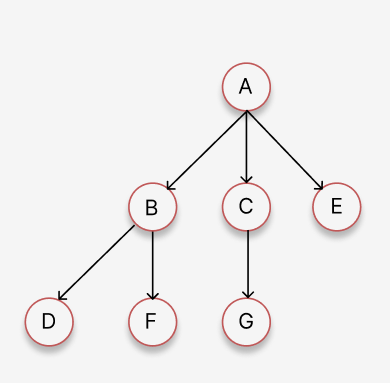
\includegraphics[height=3in]{DFS}
    \else
      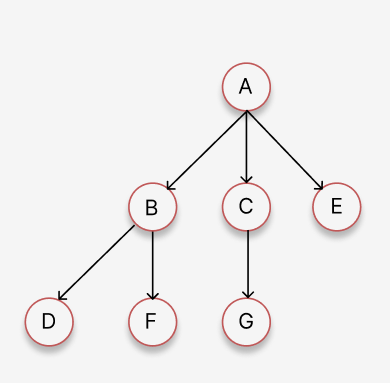
\includegraphics[bb = 92 86 545 742, height=6in]{DFS}
    \fi
    \caption{Cây đồ thị}
    \label{FigAir}
  \end{center}
\end{figure}


\section{Áp dụng thuật toán DFS vào bài toán sử dụng Prolog}
\subsection{Khởi tạo trạng thái đích}
\begin{figure}[!htbp]
  \begin{center}
    \leavevmode
    \ifpdf
      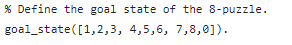
\includegraphics[height=0.5in]{DefineState}
    \else
      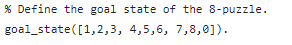
\includegraphics[bb = 92 86 545 742, height=0.5in]{DefineState}
    \fi
    \caption{Khởi tạo trạng thái đích}
    \label{FigAir}
   
  \end{center}
\end{figure}
\FloatBarrier
\subsection{Định nghĩa trạng thái di chuyển}
\begin{figure}
  \begin{center}
 \leavevmode
    \ifpdf
      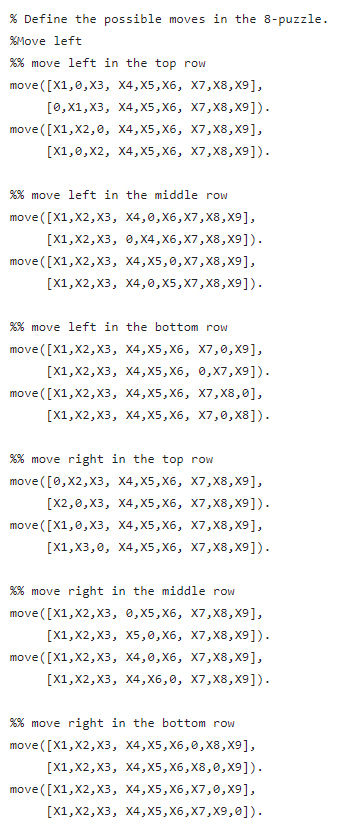
\includegraphics[height=8in]{MoveLeftRight}
    \else
      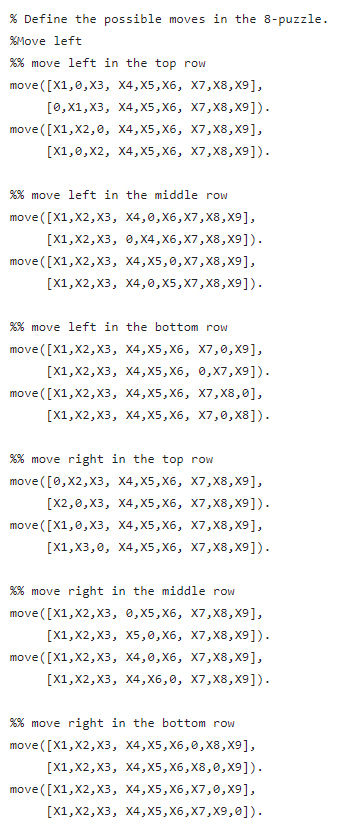
\includegraphics[bb = 92 86 545 742, height=8in]{MoveLeftRight}
    \fi
    \caption{Định nghĩa di chuyển trái và phải}
    \label{FigAir}
 \end{center}
\end{figure}
\FloatBarrier

\begin{figure}
  \begin{center}
    \leavevmode
    \ifpdf
      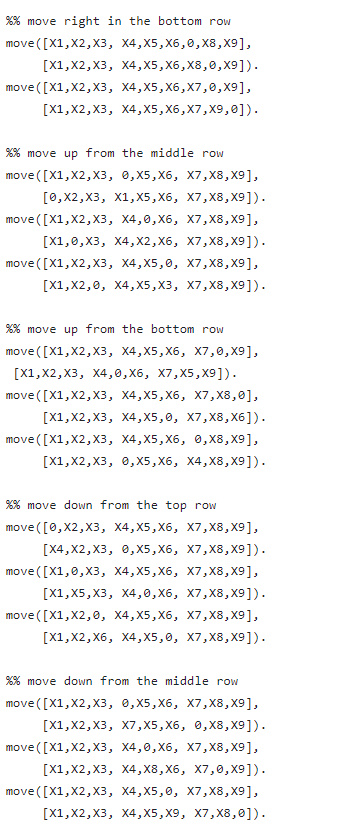
\includegraphics[height=8in]{MoveUpDown}
    \else
      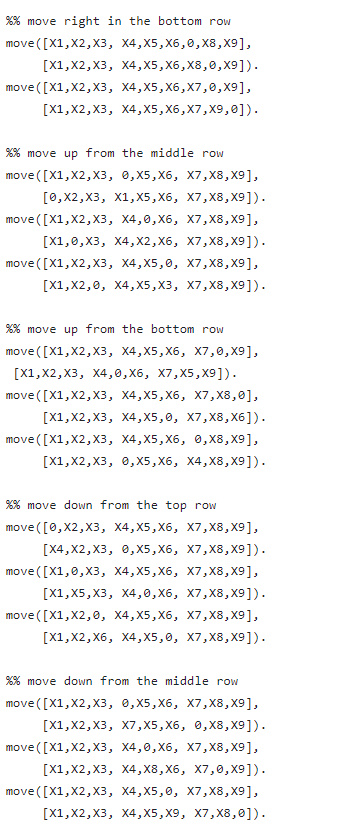
\includegraphics[bb = 92 86 545 742, height=8in]{MoveUpDown}
    \fi
    \caption{Định nghĩa di chuyển lên và xuống}
    \label{FigAir}
  \end{center}
\end{figure}
\FloatBarrier
\subsection{Cài đặt thuật toán và khởi chạy}
\begin{figure}[!htbp]
\begin{center}
    \leavevmode
    \ifpdf
      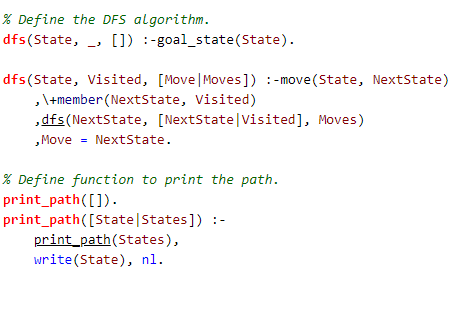
\includegraphics[height=3in]{Install}
    \else
      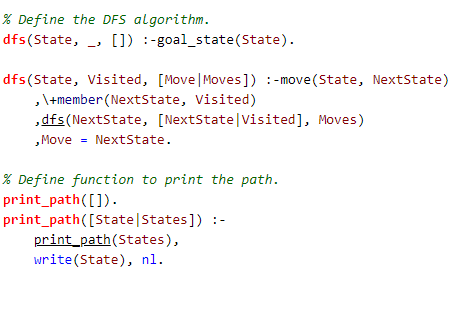
\includegraphics[bb = 92 86 545 742, height=3in]{Install}
    \fi
    \caption{Thuật toán DFS}
    \label{FigAir}
  \end{center}
\end{figure}
\FloatBarrier
\subsection{Kết quả đạt được}
\begin{figure}[!htbp]
\begin{center}
    \leavevmode
    \ifpdf
      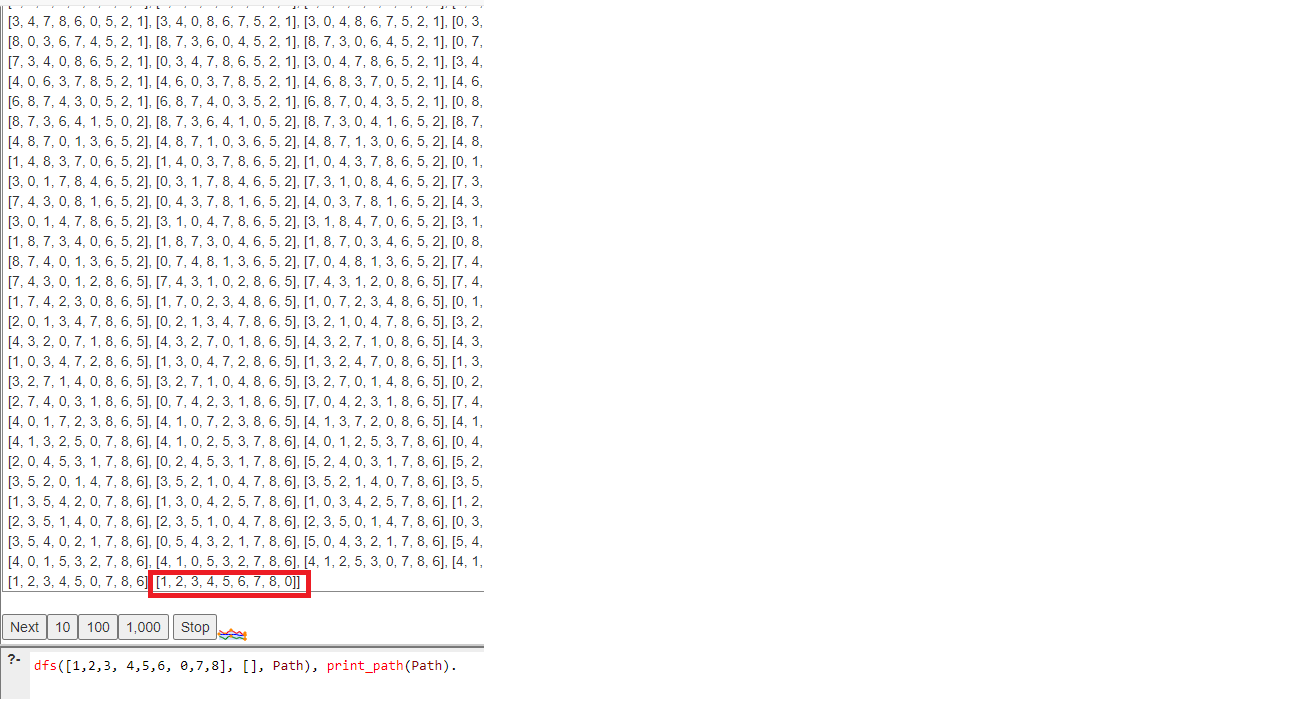
\includegraphics[height=6in]{ResultMiniSize}
    \else
      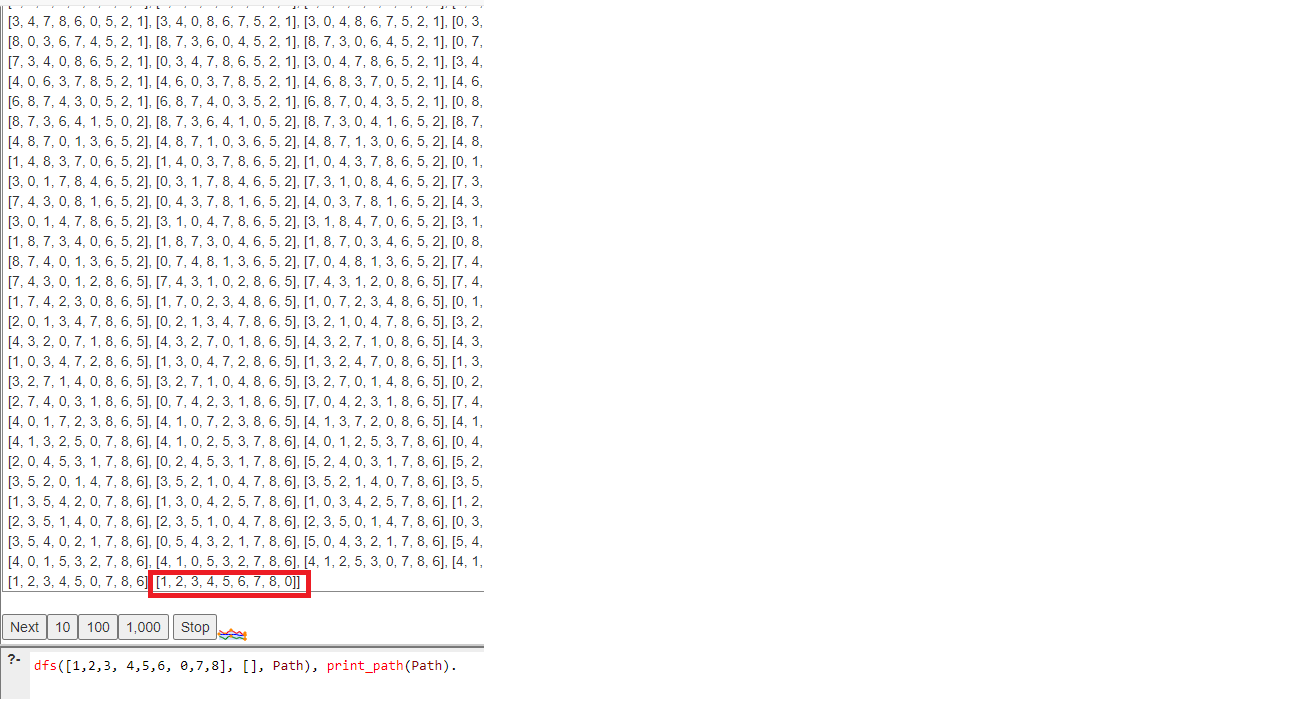
\includegraphics[bb = 92 86 545 742, height=6in]{ResultMiniSize}
    \fi
    \caption{Kết quả sau khi chạy}
    \label{FigAir}
  \end{center}
\end{figure}
\FloatBarrier


